 % !TeX spellcheck = en_US
\documentclass[12pt]{article}
\usepackage{amssymb}
\usepackage{amsmath}
\usepackage{placeins}
\usepackage{graphicx}
\usepackage[a4paper, margin=2cm]{geometry}

%opening
\title{Summary of Mathematics for the life sciences}
\author{Alberto Marin Sanguino}

\begin{document}

\maketitle
\tableofcontents

\section{The mathematics of growth}

Growth is one of the main characteristics of biological systems. All living beings grow at least during a part of their life cycle with most keeping sustained growth through it all. During biological growth, some property of the system -- size, number of individuals, biomass, radius of a tumor dots - increases with time.Lets call this property, $x$. We can indicate that x changes with time by writing it as a function $x(t)$ or as a series $x_t = x_1, x_2, x_3,\dots$ with $x_i$ being the value of x after i time units.

The simplest problems to analyze mathematically are those that happen at discrete intervals in time. For instance, if a population of microbes duplicates every hour, then the population at time $t+1$ will be twice the population at time $t$.

\begin{equation}
\label{geomgrowth_example}
x_{t+1} = 2 \, x_t
\end{equation}

so given the population at the initial time,  $x_0$, then $x_1=2\, x_0$, $x_2=2\, x_1$ and so on. We can calculate the population at time $t$ using the simple formula:

\begin{equation}
x_{t} = 2^t \, x_0
\end{equation}

this is so simple that we hardly need any math!

Now we move on to a slightly more complicated case. The radius of a tumor increases at a rate of  15 \% every hour, what is the duplication time of the tumor? The general form of equation \ref{geomgrowth_example} is

\begin{equation}
\label{geomgrowth_general}
x_{t+1} = x_t  + r \, x_t =(1 + r) \, x_t
\end{equation}

and so

\begin{equation}
\label{geomgrowth_general2}
x_{t} = (1 + r)^{t} \, x_0
\end{equation}


thi is called \textbf{geometric growth} with $r=0.15$ for our tumor. Now if the time it takes for x to duplicate is $t_d$,

\begin{equation}
2\, x_{0} = (1 + r)^{t_d} \, x_0
\end{equation}

where $x_0$ cancels out. Now we can take  logarithms and rearrange:

\begin{equation}
t_d = \frac{\log 2}{\log (1 + r) }
\end{equation}

So our doubling time for $r=0.15$ is 1.74 hours, about an hour and 45 min.

But not all individuals in a population are identical. Most of the time, biological populations have many different types of individuals. Cells differentiate into types, animals grow in different stages, microbes can form spores \dots Fortunately, we have the mathematical tools to reflect that diversity. Consider a population of parasites that reproduce through eggs. Every week, some eggs hatch and produce new parasites that in time will produce more eggs. We can easily capture the idea of our population having two different components: animals of species $x$ and eggs of species $x$ by using vectors:

\begin{equation}
\mathbf{x} =\left( \begin{array}{c} x_1 \\  x_2 \end{array} \right)
\end{equation}

A vector of dimension $n$ are just collections of $n$ ``normal'' numbers which, by the way are caller scalars. 



\subsection{Ordinary differential equations}

A differential equation is an equality involving one or more unknowns ($x$, $y$, $z$,\dots) and their derivatives. Since our unknowns have derivatives, they are not just numbers like in regular -- a.k.a. algebraic -- equations. Our unknowns are functions or, more accurately, families of functions. We can make this explicit by writing our unknowns as $x(t)$, $y(t)$, $z(t)$,\dots thus sacrificing brevity for the sake of clarity. In the text that follows, very little effort will be made to maintain consistency between these two notations and we will wantonly switch between both. Live with it.

Among all differential equations, we will be interested in the simpler type. Ordinary differential equations (ODEs) are those that do not involve partial derivatives. Our functions will only have one independent variable that almost always will be time. Moreover, we will start with linear equations.

Linear equations are those where different unknowns and their derivatives are only combined linearly. Some examples of linear equations are:

\begin{align}
	\frac{dx}{dt} \: = \: &  a \, x	\nonumber\\
	\frac{dx}{dt} + \frac{dy}{dt}\: = \: &  0 \nonumber\\
	\frac{dx}{dt} \: = \: &  a \, x + b \, y \nonumber
\end{align}

while the following equations are not linear:

\begin{align}
	\frac{dx}{dt} \: = \: &  x^2	\nonumber\\
	\frac{dx}{dt} + \frac{dy}{dt}\: = \: &  x \, y \nonumber\\
	\frac{dx}{dt} \: = \: &  \sin x \nonumber
\end{align}

Keep in mind that the linearity requirement only applies to the unknowns and not to the independent variable. The following equations are all linear


\begin{align}
	\frac{dx}{dt} \: = \: &  t^2 \, x	\nonumber\\
	\frac{dx}{dt} + \frac{dy}{dt}\: = \: &  \sin t \nonumber\\
	\frac{dx}{dt} \: = \: &  t \, x + t^2 \, y \nonumber
\end{align}

In these equations, the coefficients that multiply our unknowns just happen to be functions of time. A linear equation can have coefficients that depend on time and also have time-dependent independent terms. In general, we will not concern ourselves with such systems.

\subsection{Linear equations}

Solving differential equations is very challenging, that's why we will try to avoid it whenever possible. In fact, we are only going to solve one differential equation during the whole course. We will solve it in two versions: with one variable and with several variables.

\subsubsection{Solving the linear equation with one variable}

Lets start with the simplest possible case, which also happens to describe a fundamental biological process: exponential growth.

\begin{equation}
	\label{odexp}
	\frac{dx}{dt} = \mu \, x 
\end{equation}

Which can be read as: ``the rate of increase of a population $x$ is proportional to its own size.'' This equation is easy to solve because we can separate the variables:


\begin{equation}
	\frac{dx}{x} = \mu \, dt \nonumber
\end{equation}

and integrate

\begin{equation}
	\int \frac{dx}{x} = \mu \, \int  dt \nonumber
\end{equation}

\begin{equation}
	\ln{x} = \mu \, t + C \nonumber
\end{equation}

Since $C$ is an arbitrary constant, we can define it in terms of another constant $C= \ln{k}$ so:

\begin{equation}
	\ln{x} - \ln{k}  = \mu \, t  \nonumber
\end{equation}

Applying the well known properties of logarithms listed in appendix \ref{logprop}

\begin{equation}
	\ln{\frac{x}{k}}   = \mu \, t \nonumber
\end{equation}

exponentiating both sides and rearranging

\begin{equation}
	x   = k \, e^{\mu \, t} \nonumber
\end{equation}

This is the \emph{general solution} of the differential equation. It is a family of functions because we can generate infinite functions assigning different values to k. For every possible value of $k$ there is a \emph{particular solution} of the equation.

We are not normally interested in general solutions. General solutions are for mathematicians. We want the particular solution that fits some \emph{initial condition}, $x(0)$, often written $x_0$. For instance, we have a bacterial culture that starts with an optical density of 0.01. How do we find the right value for k?


\begin{equation}
x(0) = 0.01 \Rightarrow	 k \, e^{\mu \, 0} = 0.01 \Rightarrow	k=0.01 \nonumber
\end{equation}

In general, we use the solution to the exponential equation as:

\begin{equation}
	x   = x_0 \, e^{\mu \, t} \nonumber
\end{equation}

\subsubsection{Solving the linear equation with several variables}


Our simple linear equation can also have more that one variable:

\begin{align}
	\label{odenvar}
	\frac{dx_1}{dt} =& a_{1,1} \, x_1 + a_{1,2} \, x_2 \nonumber\\
	\frac{dx_2}{dt} =& a_{2,1} \, x_1 + a_{2,2} \, x_2
\end{align}

when dealing with several variables, it helps a lot to use vectors and matrices.

\begin{equation}
	\frac{d}{dt} \begin{pmatrix} x_1\\ x_2 \end{pmatrix} = \begin{pmatrix} a_{1,1} & a_{1,2}\\ a_{2,1} & a_{2,2} \end{pmatrix} \begin{pmatrix} x_1\\ x_2 \end{pmatrix} \nonumber
\end{equation}

Thus, we can write any equation with n variables as:

\begin{equation}
	\label{odenvar_mat}
	\frac{d\mathbf{x}}{dt}  = \mathbf{A} \, \mathbf{x}
\end{equation}

Note that vectors and matrices are written in boldface.

Since the solution of the equation for one variable was an exponential, lets make the hypothesis that an exponential can also be a solution for this case. We assume

\begin{equation}
	\mathbf{x}= \mathbf{v} \, e^{\lambda \, t} \nonumber
\end{equation}

Since $\mathbf{x}$ is a vector now, we multiply our exponential times a  vector of constants $\mathbf{v}$. We can test if this is a valid solution by substituting it into the equation, which gives:

\begin{equation}
	\frac{d}{dt} \left( \mathbf{v} \, e^{\lambda \, t} \right)  = \mathbf{A} \, \mathbf{v} \, e^{\lambda \, t}  \nonumber
\end{equation}

On the left hand side, the vector of  constants can be taken out of the derivative so:

\begin{equation}
	\mathbf{v} \, \frac{d}{dt} \left(  e^{\lambda \, t} \right)  = \mathbf{A} \, \mathbf{v} \, e^{\lambda \, t}  \nonumber
\end{equation}
 
 and
 
 \begin{equation}
 	\mathbf{v}   \lambda \, e^{\lambda \, t}   = \mathbf{A} \, \mathbf{v} \, e^{\lambda \, t} \nonumber
 \end{equation}
 
canceling out the exponentials:

\begin{equation}
\label{eigendefinition}
\mathbf{A} \, \mathbf{v}  = \lambda  \,	\mathbf{v}   
\end{equation}
 
So $\mathbf{x}=\mathbf{v} \, e^{\lambda \, t}$ will be a solution of the equation as long as $\lambda$ and $\mathbf{v}$ satisfy equation (\ref{eigendefinition}).

We can solve the equation and find all possible values of $\lambda$ by rearranging terms.

\begin{equation}
	\mathbf{A} \, \mathbf{v}  - \mathbf{I} \, \lambda  \,	\mathbf{v}   = 0 \nonumber
\end{equation}

note we have multiplied lambda by the identity matrix $\mathbf{I}$. This is a matrix of zeros everywhere except its main diagonal, which is occupied by ones. The identity matrix plays the same role as number one among scalars, it does not alter the matrices or vectors it multiplies. Now we can factor $\mathbf{v}$ out 

\begin{equation}
	\label{solve4eigenvec}
	\left( \mathbf{A}   - \mathbf{I} \, \lambda     \right) \, \mathbf{v} =  0  
\end{equation}

This is an homogeneous system of equations with the components of $\mathbf{v}$ as unknowns. For the system to have a solution other than the trivial, $\mathbf{v}=\mathbf{0}$, the determinant of the parenthesis must satisfy:

\begin{equation}
	\label{solve4eigenval}
	\left| \mathbf{A}   - \mathbf{I} \, \lambda     \right|  =  0  
\end{equation}

The expansion of this determinant results in a $n-th$ degree equation in terms of lambda known as the characteristic equation of the system.

\begin{equation}
c_n \, \lambda^n +c_{n-1} \, \lambda^{n-1}  + \dots  + c_1 \, \lambda + c_0 = 0 \nonumber
\end{equation}

\subsection{Eigenvalues and eigenvectors} 

\subsubsection{Real eigenvalues}
A matrix $\mathbf{A}$ with size $n \times n$ has n vectors $\mathbf{v_i}$ for $i = 1 \dots n$ called eigenvectors, and each eigenvector has an eigenvalue ($\lambda_i$) such that every pair of eigenvector and eigenvalue satisfy equation (\ref{eigendefinition}).
	
In order to understand the meaning of this and why eigenvector and eigenvalues are extremely important in applied mathematics, we have to think of the matrix product as an operation that transforms one vector into another. For instance, lets take the matrix
\begin{equation}
	\mathbf{A}  = \begin{pmatrix} -1 & -4\\ -3 & -2\end{pmatrix} \nonumber
\end{equation}

If we multiply $(1,2)$ times the matrix we obtain another vector:

\begin{equation}
	 \begin{pmatrix} -1 & -4\\ -3 & -2\end{pmatrix} \,  \begin{pmatrix} 1\\ 2\end{pmatrix}=\begin{pmatrix} -9 \\ -7\end{pmatrix}\nonumber
\end{equation}

So matrix $\mathbf{A}$ transforms  (1,2) into  (-9,-7). Now if  we transform another vector:

\begin{equation}
	\begin{pmatrix} -1 & -4\\ -3 & -2\end{pmatrix} \,  \begin{pmatrix} 4\\ -3\end{pmatrix}=\begin{pmatrix} 8 \\ -6\end{pmatrix}\nonumber
\end{equation}

In the previous case, the transformation changed the direction of our vector but now, vector (4,-3) was transformed into a stretched version of itself with double length. If we now transformed $(8,-6)$ using the matrix, we would obtain $(16,-12)$, which is again the same vector multiplied by two. So (4,-3) is an eigenvector of $\mathbf{A}$ and the corresponding eigenvalue is $\lambda=2$. Note that negative eigenvalues will change the sense of the vector but not its direction, as is the case with the second eigenvector of this matrix $(1,1)$.

\begin{equation}
	\begin{pmatrix} -1 & -4\\ -3 & -2\end{pmatrix} \,  \begin{pmatrix} 1\\ 1\end{pmatrix}=- \begin{pmatrix} 5 \\ 5\end{pmatrix}\nonumber
\end{equation}

Obviously, the corresponding eigenvalue is $\lambda=-5$.

But how can we find out the eigenvectors and eigenvalues of a matrix other than by trial and error? First we get the eigenvalues using equation \ref{solve4eigenval}:

\begin{equation}
  \left|\begin{matrix} -1-\lambda & -4\\ -3 & -2-\lambda\end{matrix} \right| = 0 \nonumber
\end{equation}

we get the characteristic polynomial

\begin{equation}
	\lambda^2  +3 \,  \lambda  - 10 = 0 \nonumber
\end{equation}

A primary school problem we can solve:

\begin{equation}
	\lambda= \frac{-3 \pm \sqrt{9+40}}{2} \nonumber
\end{equation}

with two solutions $\lambda_1=-5$ and $\lambda_2=2$. We have already seen that the eigenvector $\mathbf{v_1}$ for $\lambda_1$ is . Can we find the other one? We can go back to equation (\ref{eigendefinition}) or use the already factored out version in equation  (\ref{solve4eigenvec})

\begin{equation}
\begin{pmatrix} -1-\lambda & -4\\ -3 & -2-\lambda\end{pmatrix} \, \begin{pmatrix} v_x \\  v_y\end{pmatrix} = 0 \nonumber
\end{equation}

For the case $\lambda = 2$:

\begin{equation}
	\begin{pmatrix} -3 & -4\\ -3 & -4\end{pmatrix} \, \begin{pmatrix} v_x \\  v_y\end{pmatrix} = 0 \nonumber
\end{equation}

\begin{align*}
	-3 \, v_x - 4 \, v_y =& 0 \nonumber\\
	-3 \, v_x - 4 \, v_y =& 0 \nonumber
\end{align*}

Which is the same equation twice, so there is no unique solution. This shows a very important property of eigenvectors: they are never unique. It is easy to see that v=(4,-3) cancels out the equation. If we had just chosen $v_x=1$, then our eigenvector would have been $\mathbf{v}=\left( 1,\frac{-3}{4} \right)$.

Now we can do the same for  $\lambda = -5$:

\begin{align*}
	4 \, v_x - 4 \, v_y =& 0 \nonumber\\
	- 3 \, v_x  + 3 \, v_y =& 0 \nonumber
\end{align*}

This is actually the same equation twice. It is easy to see that whenever $v_x=v_y$, both equations will be satisfied, so we can choose $\mathbf{v} = (1, 1)$.

\paragraph{Exercise:} Can you use equation (\ref{eigendefinition}) to show that given an eigenvector $\mathbf{v}$ and a constant $k$, any vector $k \, \mathbf{v}$ will also be an eigenvector?

\subsubsection{Complex eigenvalues}

Now lets analyze another matrix 

\begin{equation}
	\mathbf{A}  = \begin{pmatrix} 0 & -1\\ 1 & 0\end{pmatrix}  \nonumber
\end{equation}

Characteristic polynomial

\begin{equation}
	\lambda^2 + 1 = 0 \nonumber
\end{equation}

The solutions to this equation are imaginary $\lambda_1 = i$ and $\lambda_1 = -i$.

Complex eigenvalues always come in conjugate pairs: $\lambda_1 = a + b\, i$,  $\lambda_2 = a - b\, i$. In the context of ODEs, The real parts of a complex eigenvalue determine the stability, just as real eigenvalues do, while the existence of imaginary parts involves the existence of oscillations. Note that imaginary eigenvalues can only appear for systems with two or more variables. This means that for a system to oscillate, it must have at least two variables.


\subsection{General solutions for linear equations}

So putting together all the eigenvectors of the system and the corresponding eigenvalues, we get the general solution for our equation with n variables:


\begin{equation}
	\label{odenvar_mat_sol}
	\mathbf{x}= c_1 \, \mathbf{v_1} \, e^{\lambda_1 \, t} + c_2 \, \mathbf{v_2} \, e^{\lambda_2 \, t} +  \dots + c_n \, \mathbf{v_n} \, e^{\lambda_n \, t} 
\end{equation}

Where $c_1 \dots c_n$  are arbitrary constants, the ones that can be used to adjust initial values. Each vector $\mathbf{v_i}$ and its corresponding constant $\lambda_i$ are called eigenvector and eigenvalue respectively.


When the eigenvalues (and eigenvectors) are complex, the solutions described above will be complex. But we are not interested in complex solutions, since all our models have real variables. To see how complex eigenvalues cause oscillations in real solutions, lets see a combination of complex exponentials:

\begin{equation}
	x_1= c_1 e^{\left(  a + b\, i\right) \, t} + c_2 \,  e^{\left(  a + b\, i\right)\, t} = 
	c_1  \, e^{a \, t} \, e^{ i \, b \, t} + c_2 \,  e^{a \, t} \, e^{-i \, b \, t} 
	\nonumber
\end{equation}

factoring out the real exponential

\begin{equation}
x_1= e^{a \, t} \,  \left( c_1  \, e^{ i \, b \, t} + c_2 \,  e^{-i \, b \, t}\right) \nonumber
\end{equation}

Using Euler's formula:

\begin{equation}
	\label{euler}
	e^{i \theta} = cos \theta + i \, \sin \theta 
\end{equation}

\begin{equation}
	x_1= e^{a \, t} \,  \left( c_1  \, \left(  \cos{ b \, t} + i \, \sin{ b \, t} \right)+ c_2 \, \left( \cos{- b \, t} + i \, \sin{- b \, t} \right) \right) \nonumber
\end{equation}

\begin{figure}
\begin{center}
	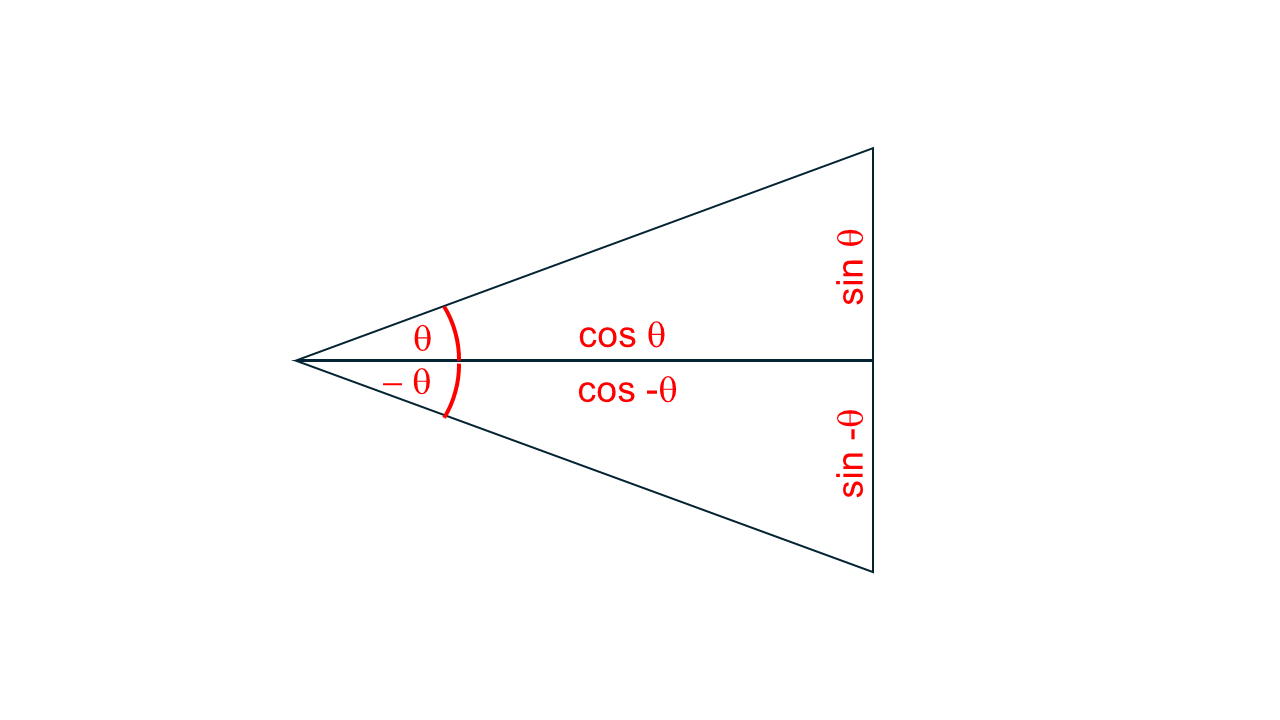
\includegraphics[width=\textwidth]{trigo}
\end{center}
\caption{Some basic trigonometric relations.}
\label{fig:trigo}
\end{figure}

As can be seen in  figure \ref{fig:trigo}, $- \sin{b \, t}=\sin{- b \, t}$ and $\cos{b \, t}=\cos{ - b \, t}$ so we can rearrange terms:

\begin{equation}
	x_1= e^{a \, t} \,  \left( c_1  \, \left(  \cos{ b \, t} + i \, \sin{ b \, t} \right)+ c_2 \, \left( \cos{ b \, t} - i \, \sin{ b \, t} \right) \right) \nonumber
\end{equation}


\begin{equation}
	x_1=   \left( c_1+c_2\right) \, e^{a \, t} \, \cos{ b \, t}  + i \, \,\left( c_1-c_2 \right) \,e^{a \, t} \,   \sin{ b \, t}   \nonumber
\end{equation}

Note that this solution has the form $x_1(t) = u(t) + i \, v(t)$ where both $u(t)$ and $v(t)$ are real functions. Moreover, these functions are linearly independent so a combination of both will be a proper general solution. By defining new arbitrary constants, we will get the general solution that includes al possible real solutions of the equation:

\begin{equation}
	x_1=   e^{a \, t} \,  \left(  A  \, \cos{ b \, t}  +  B  \,   \sin{ b \, t}  \right) \nonumber
\end{equation}

So the real part of our solutions will be the product of an exponential and an oscillatory function. Moreover, the exponential depends only on the real part of the eigenvalue, $\operatorname{Re}(\lambda) = a$, while the oscillations depend on its imaginary part,  $\operatorname{Im}(\lambda) =b$ (see figure \ref{fig:cmplxeigen}). 

\begin{figure}
	\begin{center}
		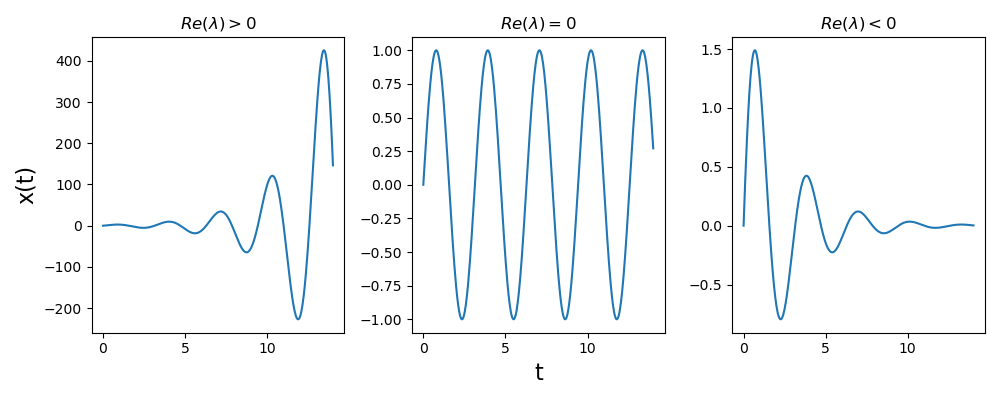
\includegraphics[width=\textwidth]{complex_eigen}
	\end{center}
	\caption{Overal behavior of solutions when eigenvalues are complex. The sign of $\operatorname{Re}(\lambda)$ determines stability and $\operatorname{Re}(\lambda)$ governs oscillations}
	\label{fig:cmplxeigen}
\end{figure}


\FloatBarrier

\subsection{Differential equations of higher order}

The following differential equation:

\begin{equation}
	 \frac{d^2x}{dt^2} = \frac{k}{m} \, x - g \nonumber
\end{equation}

is called a second order differential equation because it contains a second derivative. This equation can lead to oscillations, even though, we just said only systems with two variables can show this behavior. The reason for that is that any  differential equation of order $n$ can be written as a first order differential equation with n variables. If we add the variable $y(t)$ as the derivative of $x(t)$ to the equation above, it becomes:

\begin{align}
	\frac{dx}{dt} =& \: y \nonumber \\
	\frac{dy}{dt} =& \: \frac{k}{m} \, x - g \nonumber
\end{align}


\subsection{Plotting solutions}

The particular solutions of a differential equation can be plotted as each variable being a function of time as shown in figure \ref{fig:cmplxeigen}, but there are alternative representations. A frequently used plot is the phase space like the one shown in figure \ref{fig:phase_plane}. In this plot, the state variables of the system are used as axes. Since time is not explicitly included in the plot, the lines showing the evolution of the system have arrows that indicate the direction in which the system moves as time goes by. In a plot like this, several particular solutions can be shown at the same time, the line representing each solution is called an orbit. 
\begin{figure}
	\begin{center}
		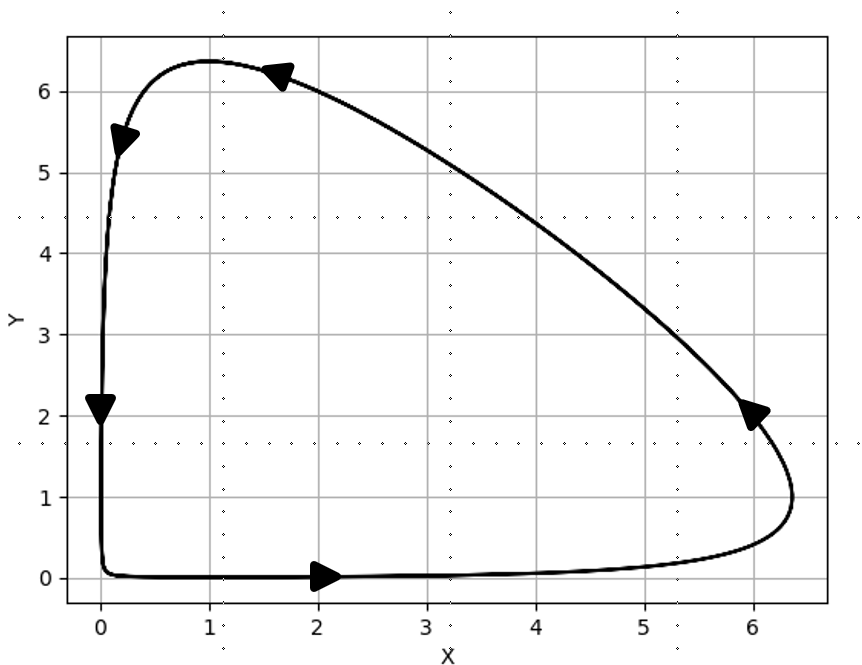
\includegraphics[width=0.7\textwidth]{phase_plane}
	\end{center}
	\caption{Phase plane representation of a particular solution of a two variable oscillatory system.}
	\label{fig:phase_plane}
\end{figure}

\subsection{Non-linear systems}

Unlike linear equations, non-linear equations rarely have analytic solutions. fortunately, we can extract a lot of information from a differential equation without solving it. This is so because we are often not interested in every detail about its dynamics but rather on its long term behavior.

\subsubsection{Steady states}

The first step to analyze non-linear systems is to find out its steady states. for a given non-linear system:

\begin{equation}
	\label{odegeneral}
	\frac{d\mathbf{x}}{dt} = \mathbf{f}(\mathbf{x})
\end{equation}

we can calculate its steady states as those values $\mathbf{x}= \mathbf{x_0}$ such that:

\begin{equation}
	\label{stst}
	\mathbf{f}(\mathbf{x_0}) = 0
\end{equation}

Steady states are important because once the system reaches it, it will remain in it as long as it is not perturbed.

\paragraph{Example:} Lets take another growth equation:

\begin{equation}
	\label{odgrowth}
	\frac{dx}{dt} = \mu(x) \, x 
\end{equation}

Unlike exponential growth, where $\mu$ is constant, his more general form makes the growth rate dependent on the size of the population. This makes the model more realistic as resources are expected to become scarce once the population density becomes too high. A particular case is that of logistic growth, where $\mu(x) = \mu_{m} (1 - x / K)$. Our equation becomes

\begin{equation}
	\label{logistic}
	\frac{dx}{dt} = \mu_{m} \left(1 - \frac{x}{K} \right) \, x 
\end{equation}

The steady state condition will be:

\begin{equation}
 \mu_{m} \left(1 - \frac{x}{K} \right) \, x = 0
\end{equation}

which can happen in two different ways. Either $x=0$, just like happened for exponential growth, or $x=K$.

\begin{figure}
	\begin{center}
		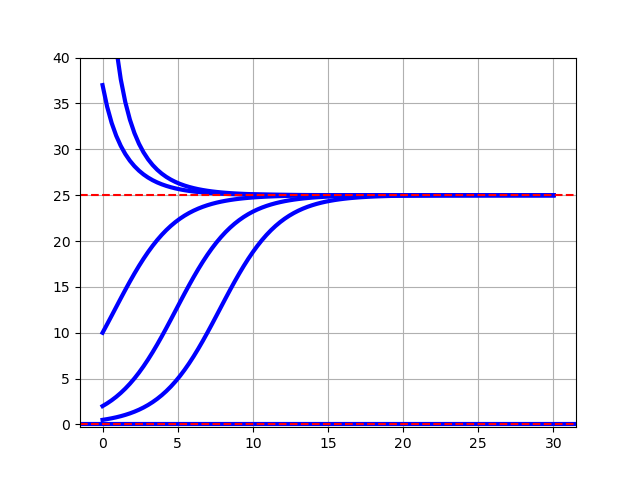
\includegraphics[width=0.8\textwidth]{logisticall}
	\end{center}
	\caption{Logistic growth model with $K=25$, the two steady states $x=0$ and $x=25$ are marked with red dashed lines. It can clearly be seen that the system tends to move away from one steady state and towards the other.}
	\label{fig:logisticall}
\end{figure}

\subsubsection{Stability}

Figure \ref{fig:logisticall} shows how the behavior of the logistic equation is dictated by its two steady states. The system tends to move away from $x=0$, which is therefore called an \emph{unstable steady state} or \emph{repulsor} and towards $x=K$, which is a \emph{stable steady state} or \emph{attractor}. But how do we know whether a steady state is stable?

A steady state is said to be stable when the system tends to return to it after being moved away from it. In other words, lets assume a system has a steady state at $x=x_0$ and we move the system to another, nearby state $x_0+\delta x$. $\delta x$ is a small number and we call it a perturbation. if we define our variable as a composition of the steady state and a time varying perturbation: $x(t) = x_0 + \delta x(t)$, the system can be said to be stable if $\delta x \rightarrow 0$ as $t \rightarrow \infty$. Conversely, we say the system is unstable if $\delta x \rightarrow \infty$ as $t \rightarrow \infty$.  But how can we predict the behavior of $\delta x$? since we can only solve linear systems, we will have to turn this into a linear equation \dots

\subsubsection{Linearization}

Making the change of variable $x(t) = x_0 + \delta x(t)$ in equation \ref{odegeneral},

\begin{equation}
	\frac{d}{dt} \left( x_0 + \delta x(t) \right) = f(x_0 + \delta x(t)) \nonumber
\end{equation}

The left hand side is the  derivative of a sum and can be rewritten as the sum of derivatives. Moreover, since $\delta x$ is small by definition, we can approximate this as a linear system as shown in equation \ref{TaylorLin}.

\begin{equation}
	 \frac{dx_0}{dt} + \frac{d}{dt}\delta x(t)  = f(x_0) +\left|\frac{df}{dx}\right|_0 \, \delta x(t)) \nonumber
\end{equation}

$x_0$ is constant, so $\frac{dx_0}{dt}=0$ and $f(x_0)=0$ by the definition of steady state. This leaves the system 

\begin{equation}
	\label{svl}
	\frac{d}{dt}\delta x(t)  =  \left|\frac{df}{dx}\right|_{x=x_0} \,  \delta x(t)) 
\end{equation}

Equation \ref{svl} is called variational linearized system and it is easily to solve. If $\left|\frac{df}{dx}\right|_0 < 0$ then $\delta x \rightarrow 0$ and the steady state is stable. If $\left|\frac{df}{dx}\right|_0 > 0$, $\delta x \rightarrow \infty$ and the system is unstable.

\paragraph{Example:} In the logistic equation:

\begin{equation}
\frac{df}{dx} = \mu_{m} \left( 1-\frac{2 x}{K}\right) \nonumber
\end{equation}

 So for the steady state $x=0$, the l.v.s. is:
 
 \begin{equation}
 	\frac{d}{dt}\delta x(t)  = \mu_m \,  \delta x(t))  \nonumber
 \end{equation}
The solution to this equation is a positive exponential so the perturbation $\delta x(t)$ will be amplified with time. This means the steady state is unstable.

and for the steady state $x=K$:

 \begin{equation}
	\frac{d}{dt}\delta x(t)  = -  \mu_m \,  \delta x(t))  \nonumber
\end{equation}Since the solution of this equation is a negative exponential, any perturbation will fade with time and the steady state is stable.

For systems with more variables:

\begin{align}
	\frac{dx}{dt}=&f_x(x,y)  \nonumber\\
	\frac{dy}{dt}=&f_y(x,y)  \nonumber
\end{align}

the l.v.s. looks like this

 \begin{equation}
 	\label{fig:svlnvar}
	\frac{d}{dt} \begin{pmatrix} \delta x\\ \delta y \end{pmatrix}= \begin{pmatrix} \frac{\partial f_x}{\partial x} & \frac{\partial f_x}{\partial y}\\ \frac{\partial f_y}{\partial x} & \frac{\partial f_y}{\partial y} \end{pmatrix} \, \begin{pmatrix} \delta x\\ \delta y \end{pmatrix}
\end{equation}

Again, the Jacobian matrix contains the partial derivatives evaluated at the steady state, so it is a matrix of constants.

\paragraph{Example:} The chemical signaling system in figure \ref{fig:signalpathd} has two components $X$ and $R$ which responds to an input signal $S$:

\begin{align}
	\frac{dR}{dt} =&\: k_1 \, S - k_2 \, X \, R  \nonumber\\
	\frac{dX}{dt} =&\: k_3 \, S - k_4 \, X  \nonumber
\end{align}

\begin{figure}
	\begin{center}
		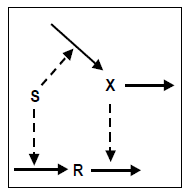
\includegraphics[width=0.3\textwidth]{signalpathd}
	\end{center}
	\caption{A signaling pathway with input $S$ and output $R$. }
	\label{fig:signalpathd}
\end{figure}

The system has a steady state at:

\begin{align}
	R =&\: \frac{k_1 k_4}{k_2 k_3}  \nonumber\\
	X =&\: \frac{k_3}{k_4}S \nonumber
\end{align}

and the jacobian matrix:

\begin{equation}
\mathbf{J} =	 \begin{pmatrix} - k_2 \, X &  - k_2 \, R \\   0  & -k_4 	\end{pmatrix} \nonumber
\end{equation}

Since we are interested in a particular steady state, we substitute its value in the jacobian matrix to obtain the linearized system:

\begin{equation}
\frac{d}{dt}	 \begin{pmatrix} \delta R \\ \delta S	\end{pmatrix} =	 \begin{pmatrix} - \frac{k_2 k_3}{k_4}S &  - \frac{k_1 k_4}{k_3} \\   0  & -k_4 	\end{pmatrix} \begin{pmatrix} \delta R \\ \delta S	\end{pmatrix} \nonumber
\end{equation}

And we calculate eigenvalues:

\begin{equation}
\left| \begin{matrix} - \frac{k_2 k_3}{k_4}S - \lambda &  - \frac{k_1 k_4}{k_3} \\   0  & -k_4-\lambda 	\end{matrix} \right|=0 \nonumber
\end{equation}

to obtain the characteristic polynomial
\begin{equation}
	\lambda^2 + \left( k_4 + \frac{k_2 k_3}{k_4}S \right) \, \lambda +k_2 k_3 S=0 \nonumber
\end{equation}

The solutions are $\lambda_1 = -k_4$ and $\lambda_2=-\frac{k_2 k_3}{k_4}S$. Since kinetic constants and concentrations are always positive, this system will always be stable.
\paragraph{Example} A chemostat is a microbial culture fed with fresh medium at a constant rate while the fermentation broth flows out of the culture at identical rate to keep constant volume. This system is described by the equations:

\begin{align}
	\frac{dx}{dt}=&\: \left( \mu_M \frac{s}{s+K_s} - D\right) \, x  \nonumber\\
	\frac{ds}{dt}=&\: D\, (s_0-s)-\frac{\mu_M}{Y} \frac{s}{s+K_s}\,x \nonumber
\end{align}
where $D$ is the dilution rate, $\mu_M$ the maximum growth rate and $Y$ the yield in grams of biomass produced per gram of substrate consumed.

This system has two steady states: $x=0$, $s=s_0$ and when the growth rate is equal to the dilution rate:

 \begin{equation}
	D = \mu_M \frac{s}{s+K_s} = \mu(s) \nonumber
\end{equation}

which results in 

\begin{align}
	s=& \frac{D \, K_s}{\mu_M - D} \nonumber \\
	x=& Y \, \left( s_0 - \frac{D \, K_s}{\mu_M - D} \right) \nonumber
\end{align}

The partial derivatives for the Jacobian matrix are:

\begin{align}
	\frac{\partial f_x}{\partial x }=&\:   \mu(s) - D  \nonumber\\
	\frac{\partial f_x}{\partial s }=&\: \mu_M \frac{K_s}{(s+K_s)^2} \, x   \nonumber\\
	\frac{\partial f_s}{\partial x }=&\: - \frac{\mu(s)}{Y}  \nonumber\\
	\frac{\partial f_s}{\partial s }=&\: - D -   \frac{\mu_M}{Y} \frac{K_s}{(s+K_s)^2} \, x  \nonumber
\end{align}

to analyze the stability of the first steady state, we substitute the values $x=0$, $s=s_0$ in the parrtial derivatives:

\begin{align}
	\frac{\partial f_x}{\partial x }=&\:    \mu(s_0) - D  \nonumber\\
	\frac{\partial f_x}{\partial s }=&\: 0  \nonumber\\
	\frac{\partial f_s}{\partial x }=&\:  - \frac{\mu(s_0)}{Y} \nonumber\\
	\frac{\partial f_s}{\partial s }=&\: - D   \nonumber
\end{align}

We can obtain the eigenvalues from:
 \begin{equation}
\left| \begin{matrix}  \mu(s_0) - D - \lambda  & 0\\   - \frac{\mu(s_0)
	}{Y}  &  - D- \lambda
\end{matrix} \right| = 0 \nonumber
\end{equation}

The characteristic polynomial for this case is:

 \begin{equation}
	\lambda^2 + \left( 2 D - \mu(s_0)\right) \lambda  +D^2-D \mu(s_0) = 0  \nonumber
\end{equation}

Resulting in the eigenvalues $\lambda_1 = -2 D$ and $\lambda_2 = 2\,(\mu(s_0) - D)$. Remember that the condition for a steady state to be stable is that all their eigenvalues are negative. So the steady state $x=0$,$s=s_0$ is only stable if $D > \mu(s_0)$. In other words, $\mu(s_0)$ is the highest growth rate the cells can achieve in the chemostat because $s_0$ if the highest concentration of substrate. If the dilution rate is higher than such growth rate, the cells will be washed out until $x=0$, and with no cells to consume it, the substrate concentration in the tank will be the same as in the feed.



\clearpage
\appendix
\section{Taylor Polynomial}
A polynomial can adopt practically any shape. That's why many functions can be approximated by polynomials, at least, within a certain region.

\begin{figure}[htb]
	\begin{center}
		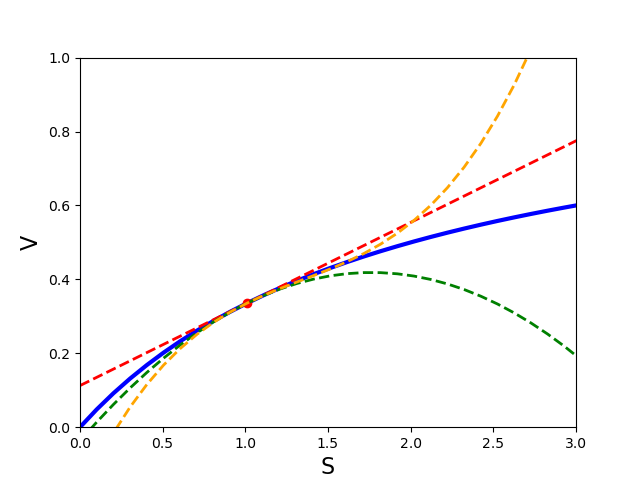
\includegraphics[width=0.6\textwidth]{MMapprox}
	\end{center}
	\caption{Polynomial approximations (dashed lines) to a Michaelis-Menten kinetics (solid blue line). Linear approximation (red) second degree (green) and third degree (orange).}
	\label{fig:MMapprox}
\end{figure}

Figure \ref{fig:MMapprox} shows the following function

\begin{equation}
	V=\frac{S}{2+S} \nonumber
\end{equation}

If we want to approximate this function with a polynomial, we have to start choosing a reference point ($S_0=1$). Whatever approximation we choose will exactly reproduce the function at the reference point. The approximation will lose quality as we move farther from this reference point. The three examples shown in the figure are polynomials of first, second and third degree in red, green and orange respectively. The  equations of the polynomials are:

\begin{align}
	V=& 0.115 + 0.221 \, S\nonumber\\
	V=& -0.032 + 0.515 \, S - 0.147 S^2\nonumber\\
	V=& -0.178 + 0.953 \, S- 0.585 S^2+ 0.146 S^3 \nonumber
\end{align}

For values in the interval $0.75 \leq S \leq 1.25$ all three approximations are very good but as we move away from the reference point, the approximations diverge. In general, higher degree polynomials are more flexible and will have better chances to approximate complicated functions, but this is not always so. In this case, for instance, we can see the second degree polynomial makes a pretty good job for $0.1 \leq S \leq 1.5$ while the third degree polynomial improves the approximation on the higher end but performs worse for $S < 1$.

Since all polynomials have the same structure, finding an approximating polynomial is just a matter of finding the numerical values for each of its coefficients. The Taylor polynomial is one way of finding out the desired coefficients. The concept is very simple. Knowing the value of a function $f(x)$ at the reference point $x_0$ and all the successive derivatives evaluated at that point, the polynomial, at an arbitrary point $x$ will be:

\begin{equation}
	T(x)=f(x_0) + \left|\frac{df}{dx}\right|_0 \left( x - x_0\right)+ \left|\frac{d^2f}{dx^2}\right|_0 \left( x - x_0\right)^2+ \left|\frac{d^3f}{dx^3}\right|_0 \left( x - x_0\right)^3+ \dots
	\nonumber
\end{equation}

where the symbols $\left| \cdot \right|_0$ around the derivatives mean that we are not using the whole derivative, which is a function, but its value at the reference point, which is a number.

The concept is very simple. At the reference point, $x=x_0$ and all terms will cancel out except $f(x_0)$ so the approximation will ve exact. As we move away from the reference point by an increment of x ($\Delta x = x - x_0$) we will first use the derivative to approximate the change in the function $\Delta f= \frac{df}{dx}\Delta x$ and we will refine the calculation by adding terms for each successive derivative.

In the context of this course, we will be interested in approximations very close to the reference state. In these cases, $\left( x - x_0\right) \ll 1$ and higher derivative terms, which are multiplied by higher powers of this number can be considered to be negligible:

\begin{equation}
	\label{TaylorLin}
	T(x) \approx  f(x_0) + \left|\frac{df}{dx}\right|_0 \left( x - x_0\right)
\end{equation}

so we can use the Taylor polynomial to obtain  linear approximations.

Taylor polynomials can easily generalized to more than one variable as long as we remember the concept of partial derivative. When a function has more than one variable $f(x,y)$ we can calculate a partial derivative for each one

\begin{equation}
	\frac{\partial f}{\partial x} =\frac{d}{dx} \left| f(x,y) \right|_{y=const}  \nonumber
\end{equation}

So we just derive as if our function only had one variable, for instance:

\begin{equation}
	f(x,y) = x^2 + x \, y + y^2 \nonumber
\end{equation}


\begin{equation}
	\frac{\partial f}{\partial x} = 2 \, x + y \nonumber
\end{equation}

\begin{equation}
	\frac{\partial f}{\partial y} =  x + 2 \,y \nonumber
\end{equation}

In a system with several variables, the role of the derivative is taken by a matrix of partial derivatives called the Jacobian Matrix $\mathbf{J}$.  $f(x,y)$:

\begin{equation}
	\mathbf{J} = \begin{pmatrix} \frac{\partial f}{\partial x} & \frac{\partial f}{\partial y} \end{pmatrix} \nonumber
\end{equation}

and the linear approximation is:

\begin{equation}
	\label{TaylorLin_nvar}
	\mathbf{T(x)} \approx  \mathbf{f(x_0)} + \mathbf{J} \left( \mathbf{x} - \mathbf{x_0}\right)
\end{equation}

The function in the previous example at the reference point $(x_0, y_0)=(1,2)$ would have $f(x_0, y_0)=7$, so


\begin{equation}
	T(x,y) = 7 + \begin{pmatrix} 4 & 5 \end{pmatrix} \, \begin{pmatrix} 1-x \\ 2-y \end{pmatrix} = 7 +  4- 4 x + 10-5 y  \nonumber
\end{equation}

\begin{equation}
	T(x,y) = 21 - 4 x - 5 y  \nonumber
\end{equation}

\FloatBarrier
%\section{Complex numbers}
%\FloatBarrier

\section{Some properties of logarithms}
\label{logprop}
\begin{equation}
 \log{(a \, b)} =	\log{a} + \log{b} 
\end{equation}

\begin{equation}
	\log{(a / b)} =	\log{a} - \log{b} 
\end{equation}

\begin{equation}
	\log{x^a} =a \, \log{x} 
\end{equation}

\begin{equation}
	e^{\ln{x}} = x 
\end{equation}












\end{document}
